\documentclass{article}
\usepackage{tikz}
\usepackage{amsmath,amssymb}

\begin{document}

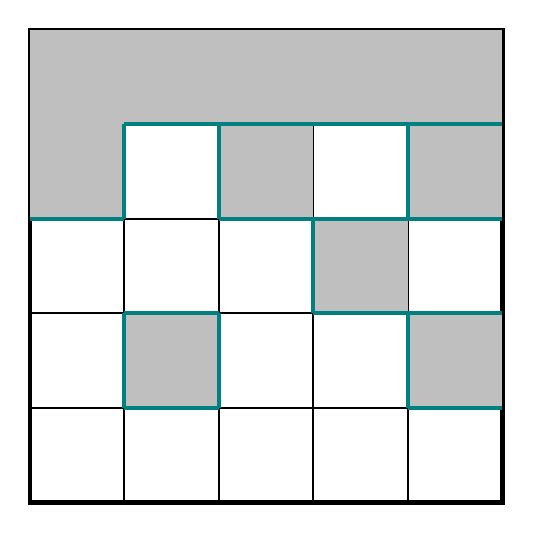
\begin{tikzpicture}[scale=1.2]
    % Draw the 5x5 grid
    \draw[thick] (0,0) grid (5,5);
    \draw[ultra thick] (0,0) rectangle (5,5);
    
    % Fill the cluster cells with gray
    \fill[gray!50] (0,3) rectangle (1,4);
    \fill[gray!50] (0,4) rectangle (1,5);
    \fill[gray!50] (1,4) rectangle (2,5);
    \fill[gray!50] (2,3) rectangle (3,4);
    \fill[gray!50] (2,4) rectangle (3,5);
    \fill[gray!50] (3,2) rectangle (4,3);
    \fill[gray!50] (3,4) rectangle (4,5);
    \fill[gray!50] (4,3) rectangle (5,4);
    \fill[gray!50] (4,4) rectangle (5,5);
    \fill[gray!50] (1,1) rectangle (2,2);
    \fill[gray!50] (4,1) rectangle (5,2);
    
    % Draw the perimeter edges in teal
    \draw[teal, line width=1.5pt] (1,1) -- (2,1);
    \draw[teal, line width=1.5pt] (1,1) -- (1,2);
    \draw[teal, line width=1.5pt] (2,1) -- (2,2);
    \draw[teal, line width=1.5pt] (1,2) -- (2,2);
    
    \draw[teal, line width=1.5pt] (4,1) -- (5,1);
    \draw[teal, line width=1.5pt] (4,1) -- (4,2);
    \draw[teal, line width=1.5pt] (4,2) -- (5,2);
    
    \draw[teal, line width=1.5pt] (3,2) -- (4,2);
    \draw[teal, line width=1.5pt] (3,2) -- (3,3);
    \draw[teal, line width=1.5pt] (4,3) -- (3,3);
    
    \draw[teal, line width=1.5pt] (4,3) -- (5,3);
    \draw[teal, line width=1.5pt] (4,3) -- (4,4);
    
    \draw[teal, line width=1.5pt] (2,3) -- (3,3);
    \draw[teal, line width=1.5pt] (2,3) -- (2,4);
    
    \draw[teal, line width=1.5pt] (0,3) -- (1,3);
    \draw[teal, line width=1.5pt] (1,3) -- (1,4);
    
    \draw[teal, line width=1.5pt] (1,4) -- (2,4);
    \draw[teal, line width=1.5pt] (2,4) -- (3,4);
    \draw[teal, line width=1.5pt] (3,4) -- (4,4);
    \draw[teal, line width=1.5pt] (4,4) -- (5,4);
\end{tikzpicture}

\vspace{0.5cm}
\noindent A cluster $\mathcal{G}(P)$ indicated in \textcolor{gray}{gray}, with size $\abs{\mathcal{G}(P)} = 11$ and \textcolor{teal}{perimeter} $\mathrm{Per}(\mathcal{G}(P)) = 19$. Note edges of the cluster running along the exterior of the grid do not contribute to the perimeter.

\end{document}